\documentclass[12pt]{article}
\usepackage{graphicx}
\usepackage{blindtext}
\usepackage{hyperref}
\title{An agent based model }
\author{ }
\begin{document}
\maketitle
\begin{abstract}
    Our model aims at representing the  voting mechanism of the main decision-making body of the Euro-system the
    governing council. Moreover, we design the discussion preceding the interest rate voting session relying on the
    following assumption: Among agents we could single out two subgroups hawks and doves, within the same group agents
    show homogenous preferences, thus we model the two groups as two agents. 
    
    
\end{abstract}
\section{Model specification}

We defined hawks as the representatives of a high-debt country who are more inclined to support higher interest rates as
means of controlling inflation. While, doves refer to individuals who are more accommodating in the monetary policy approach,
favoring lower interest rates. Moreover, we have assumed  that both agents act rationally, and that they know each
other's proposals. \par
From now on we will refer to hawks as agents in group j and doves in group i.

\vspace{8pt}
The utility function of the council voters (agent) is:
\[ U(x_i,x_{j})=-\beta_{i1}(x_i-T)^2-\beta_{i2} (x_i-N_i)^2 - ((1 - \alpha) x_i - \alpha x_j)^2\]
where:
\begin{itemize}
    \item $x_i$: is the changing rates proposed by each agent $i$
    \item $T$: is the taylor rule (Assumed to be common knowledge)
    \item $N_i$: is the agents national preferences about interest rate
    \item $\beta_{i1},\beta_{i2}$: weights assigned to taylor rule and to national preferences
    \item $x\in[-50;50] b.p.$
    \item $alpha$: the share of hawks on the total number of voters
\end{itemize}
The first term $\beta_{i1}(x_i-T)^2$ represents the disutility coming from deviations from the taylor rule prescription,
meaning the further  $x_i$ is from $T$ the higher is the disutility. The second term $ \beta_{i2}(x_i-N_i)^2$ represents
the disutility coming  from deviations from the country's national directive, meaning the further is the agent $i$ from
the country's national directive, the lower the utility. The third term $(x_i-x_j)^2$
represents the disutility coming  from deviations from the proposal of the others.
\section{Solving the model}
We solve the maximization problem of the agent i and j\par
FOC:
\[ -2\beta_{i1}(x_i-T)-2\beta_{i2}(x_i-N_i)-2(1 - \alpha) [(1 - \alpha) x_i - \alpha x_j]=0 \]
\[ \beta_{i1}x_i-\beta_{i1}T+\beta_{i2}x_i-\beta_{i2}N_i+ x_i (1 - \alpha)^2 - x_j (1 - \alpha)\alpha = 0 \]
\[ x_i = \frac{\beta_{i1} t + \beta_{i2} + x_j (1 - \alpha)\alpha}{\beta_{i1} + \beta_{i2} + (1 - \alpha)^2}\]
\[ x_j = \frac{\beta_{j1}t+\beta_{j2}N_j+ x_i (1 - \alpha)\alpha}{\beta_{j1}+\beta_{j2}+\alpha^2}\]
Solving the system of equations we derived the Nash equilibrium:
\[x_i^N = \frac{ q_i w_j + (1 - \alpha)\cdot\alpha q_j} {w_i \cdot w_j - 1}\]
\[x_j^N = \frac{ q_j w_i + (1 - \alpha)\cdot\alpha q_j} {w_i \cdot w_j - 1}\]
\begin{itemize}
    \item \(q_j = \beta_{i1} T + \beta_{i2} N_i\); \(q_i = \beta_{j1} T + \beta_{j2} N_j\)
    \item \(w_j = \beta_{1,j} + \beta_{2,j} + \alpha^2\); \(w_i = \beta_{1,i} + \beta_{2,i} + (1 - \alpha)^2\)
\end{itemize}

The Nash equilibrium suggests that the interest rate proposals of the two agents depend on their own preferences
($\beta_{1,i}$ and $\beta_{2,i}$ for agent $i$ and $\beta_{1,j}$ and $\beta_{2,j}$ for agent $j$), the Taylor rule
($T$), and the interest rate proposal of the other agent ($x_j$ for agent $i$ and $x_i$ for agent $j$).
\vspace{8pt}
The closed-form solutions for the interest rate proposals indicate that the interest rate proposals of the two agents
are linear functions of their own preferences, the Taylor rule, and the interest rate proposal of the other agent. This
suggests that the interest rate proposals of the two agents are interdependent and that they need to take into account
the actions of the other agent in order to maximize their own utility.


\subsection{Parametrization of the model}
The parameters for the hawks representative agents are set as $\beta_{1,j} = 2$ and $\beta_{2,j} = 1$, indicating that
they give more weight to the Taylor rule prescription compared to the national preferences. These hawks represent less
indebted countries, as reflected by their preference for a higher interest rate target of $N_{j} = 0.5$. On the other
hand, the doves representative agents are characterized by $\beta_{1,i} = 2$ and $\beta_{2,i} = 1.5$, indicating a
greater weight given to national preferences over the Taylor rule. The doves represent more indebted countries, and
their preference for a lower interest rate target is reflected by $N_{i} = 0$. The Taylor rule target is set to $T =
0.25$. Finally, we imposed the share of hawks $\alpha$ is equal to $60\%$. 
Based on the given parameter values, the best
reply functions of the doves and hawks are plotted to visualize the Nash equilibrium in  the graph\ref{figure1}. 
The green line indicates the best 
reply function of the doves, while the black line represents the best reply function of the hawks.
The nash equilibrium is in $(0.16,0.3)$ meaning that the qualified majority will vote for an increase of the interest
rate  about 20 b.p.
\begin{figure}
    \centering
    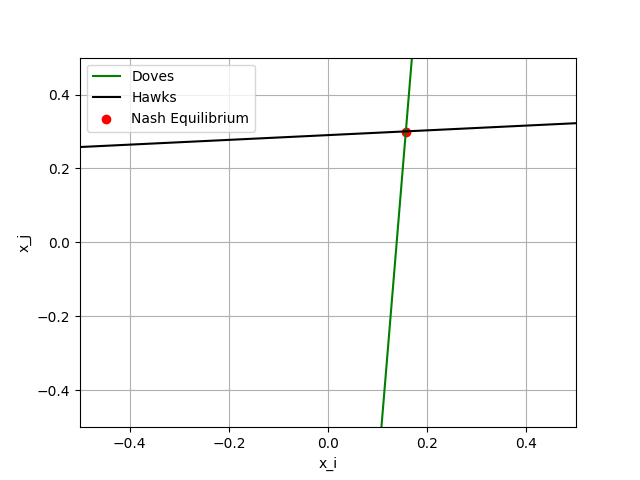
\includegraphics[scale=0.8]{plot.png}
    \caption{Nash equilibrium and best reply function\label{figure1}}
\end{figure}
\subsection{Self confirming equilibrium}
The self confirming equilibrium is the Nash equilibrium.
\subsection{Rationalisability}
\begin{table}[htbp]
    \centering
    \caption{Rationalizability Learning Steps}
    \label{table1}
    \begin{tabular}{|c|c|c|}
    \hline
    \textbf{Step} & \textbf{Doves} & \textbf{Hawks} \\ \hline
    1             & [-0.5, 0.5]      & [-0.5, 0.5]      \\ \hline
    2             & [0.35, 0.35]     & [0.1593, 0.1593]     \\ \hline
    3             & [0.35, 0.35]     & [0.1593, 0.1593]     \\ \hline
    \end{tabular}
    \end{table}
\end{document}